\newpage
\section{Bagging and Random Forests}
\label{sec:bagging-and-random-forests}

This section evaluates bagging-based tree ensembles for churn prediction. The previous section showed that a single regularized decision tree can capture useful nonlinear structure, but a single tree remains unstable because small data changes can alter the selected splits. Bagging and random forests address this weakness by fitting many trees and averaging their predictions.

The same development discipline is used as in the previous modelling sections. The held-out test set is not used. All reported results are based on stratified cross-validation inside the training set, using out-of-fold predictions where possible. The comparisons in this section are therefore development-stage comparisons of tree-ensemble variants. They identify representative ensemble candidates within the tried configurations, but they are not final test-set performance claims.

\subsection{From one tree to an ensemble}

Let a fitted decision tree produce a churn-risk score
\[
\widehat{p}(x)
=
\widehat{P}(Y=1\mid X=x).
\]
A single tree estimates this probability from the empirical churn rate in the terminal leaf reached by customer \(x\). Because each split is chosen greedily and because terminal leaf proportions can be sensitive to the training sample, single trees often have high variance.

An ensemble reduces this instability by fitting many trees and averaging their predictions. If \(B\) trees are fitted and tree \(b\) produces score \(\widehat{p}_b(x)\), the ensemble score is
\[
\widehat{p}_{\mathrm{ens}}(x)
=
\frac{1}{B}
\sum_{b=1}^{B}
\widehat{p}_b(x).
\]
The corresponding hard prediction at threshold \(t\) is
\[
\widehat{y}(x;t)
=
\mathbb{1}\{\widehat{p}_{\mathrm{ens}}(x)\geq t\}.
\]
Thus, the ensemble remains a probability-scoring classifier. Ranking metrics such as ROC-AUC and PR-AUC can be computed from \(\widehat{p}_{\mathrm{ens}}(x)\), while hard classification metrics depend on the chosen threshold.

\subsection{Bagging of decision trees}

Bagging, short for bootstrap aggregation, fits each tree on a bootstrap-resampled version of the training data. For each ensemble member \(b=1,\ldots,B\), a bootstrap sample
\[
\mathcal{D}^{*(b)}
=
\{(x_i^{*(b)},y_i^{*(b)})\}_{i=1}^{n_b}
\]
is drawn with replacement from the original training data. A decision tree \(h_b\) is fitted on this resampled dataset. Predictions are then averaged across all trees.

The main idea is variance reduction. Averaging many noisy predictors can be much more stable than using one noisy predictor. However, the reduction depends on how correlated the tree predictions are. If all trees make almost the same errors, averaging helps only a little. If the trees are diverse but still individually useful, averaging helps more.

In the bagged-tree variant used here, the base learner is a \texttt{DecisionTreeClassifier} inside scikit-learn's \texttt{BaggingClassifier}. The model uses bootstrap sampling across observations, while each tree can still consider all available features when choosing splits.

\subsection{Random forests as a bagging-based extension}

A random forest is a specialized bagging-based tree ensemble. Like plain bagging, it fits many trees on bootstrap-resampled training datasets. The additional random-forest idea is feature subsampling at each split. Instead of allowing every split to search over all \(p\) available features, each split considers only a random subset of features.

This extra randomness is designed to reduce correlation between trees. If one strong predictor dominates the split search, many bagged trees may look similar. Random feature subsampling forces different trees to explore different predictors and interactions. The ensemble average can then benefit more from diversification.

The distinction in this section is therefore not between unrelated model families. The comparison is between two tree-ensemble variants:

\begin{itemize}[leftmargin=*]
    \item \textbf{Plain bagged trees}: bootstrap-resampled decision trees where each split can consider all features.
    \item \textbf{Random forests}: bootstrap-resampled decision trees with additional random feature subsampling at each split.
\end{itemize}

\subsection{Out-of-bag observations}

Bootstrap sampling leaves out some observations from each tree's bootstrap sample. For a given tree \(b\), observations not included in \(\mathcal{D}^{*(b)}\) are called out-of-bag observations for that tree. These observations can be used to form out-of-bag predictions, because they were not used to train that particular tree.

Out-of-bag diagnostics are useful for tree ensembles because they provide an internal validation signal. In this project, however, out-of-bag scores are treated as supplementary diagnostics rather than as the main selection criterion. The main development comparisons still use the same stratified cross-validation framework as the earlier model sections, so that model-family results remain comparable.

\subsection{Hyperparameter tuning strategy}

Several valid strategies exist for hyperparameter tuning. Examples include fixed grid search, random search, Bayesian or Optuna-style optimization, successive halving, repeated cross-validation, and nested cross-validation. These strategies answer slightly different practical questions and have different computational costs.

This section uses transparent fixed grids. This choice is deliberate. The purpose here is model-family learning and controlled development-stage comparison, not final exhaustive optimization. A fixed grid makes it easy to see how the number of trees, bootstrap sample size, tree depth, leaf size, and feature subsampling affect performance. Later, after all model families have been studied, stronger training-only comparison procedures such as repeated cross-validation, paired comparisons, nested cross-validation, or more adaptive search can be used for serious final candidates.

The selected rows in this section should therefore be interpreted as the strongest configurations within the tried development grids, not as globally optimal hyperparameters and not as statistical proof of superiority.

\subsection{Experimental design}

The experiments compare four relevant models:

\begin{itemize}[leftmargin=*]
    \item the selected single decision tree from Section~\ref{sec:decision-trees};
    \item a plain bagged-tree ensemble selected from a fixed development grid;
    \item a default random forest with 100 trees;
    \item a random forest selected from a fixed development grid.
\end{itemize}

PR-AUC remains the primary development ranking metric because churn is the minority class and positive-class retrieval is central to the project. Balanced accuracy and \(F_1\) are retained as secondary threshold-dependent summaries. The final model selection stage will later revisit the strongest candidates across model families using a more careful training-only comparison.

\subsection{Bagging grid results}

Figure~\ref{fig:bagging-pr-auc-by-estimators} shows the bagged-tree grid from the perspective of PR-AUC. The results are stable across the evaluated ensemble sizes. Increasing the number of trees from 50 to 100 and 200 produces only small changes, which indicates that the ensemble has already largely stabilized within this range.

\begin{figure}[H]
\centering
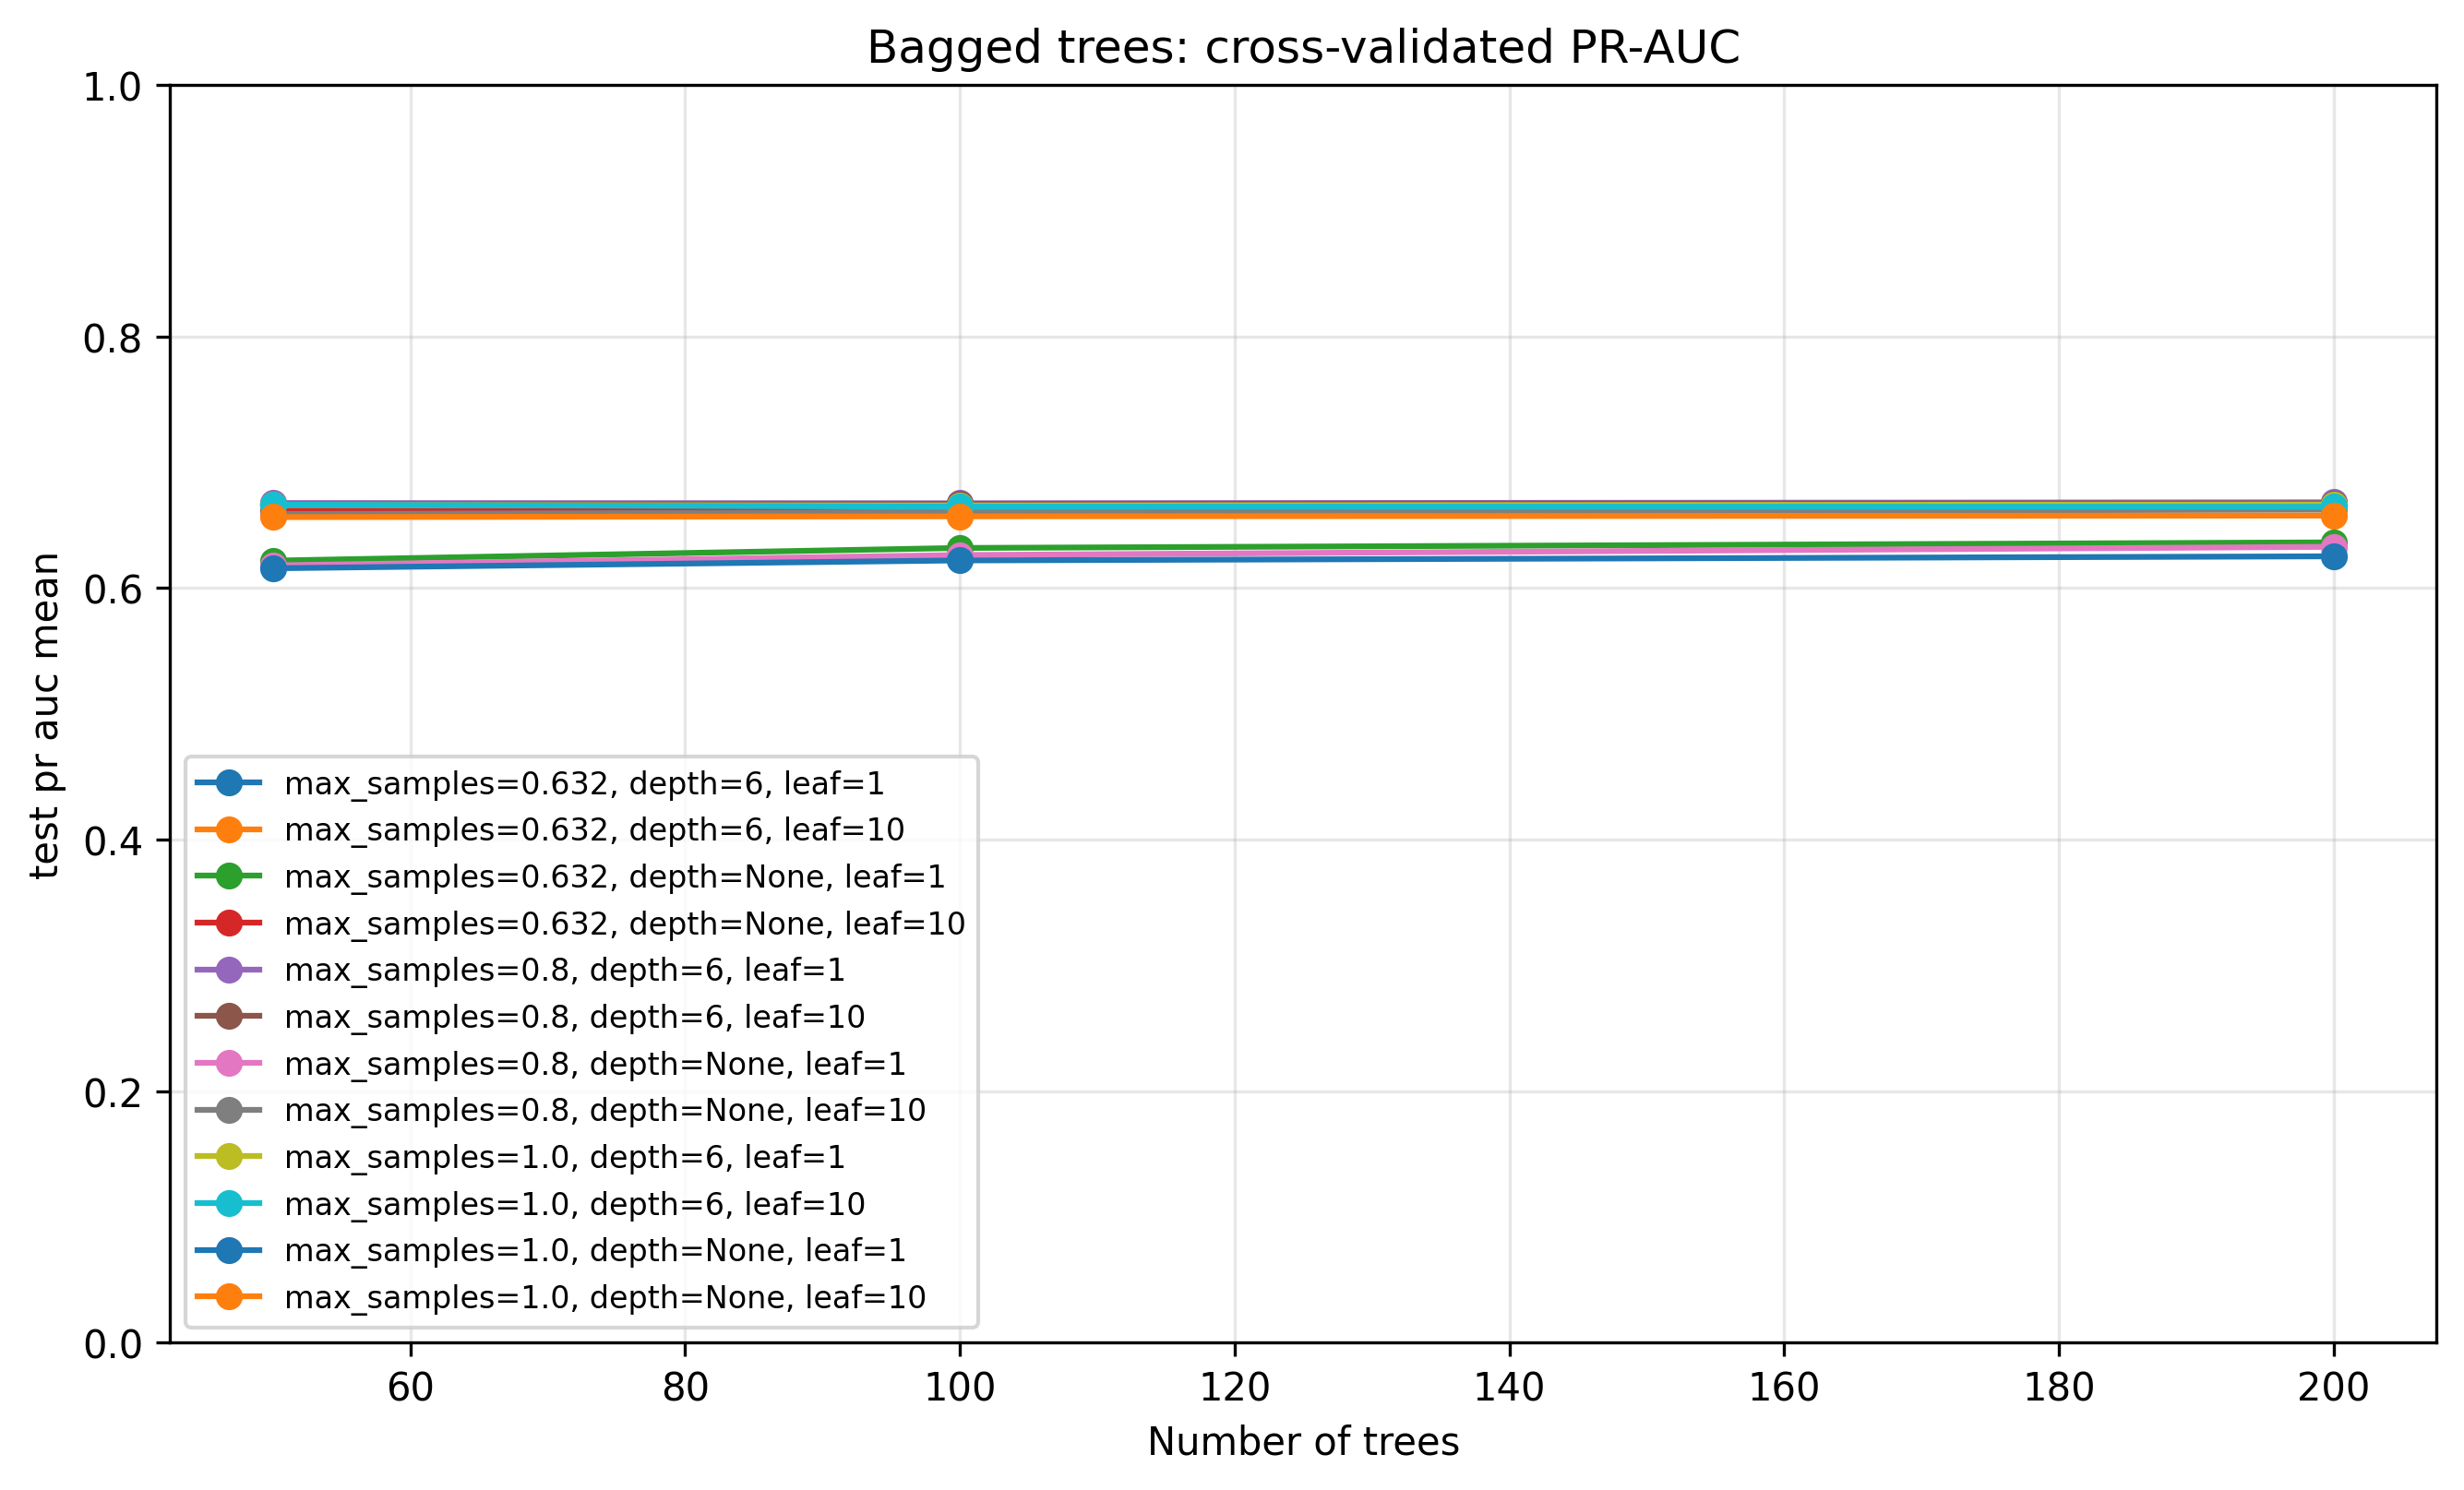
\includegraphics[width=0.88\textwidth]{../figures/bagging_pr_auc_by_estimators.png}
\caption{Bagged trees: cross-validated PR-AUC by number of trees}
\label{fig:bagging-pr-auc-by-estimators}
\end{figure}

The best bagged-tree candidate in the fixed grid uses 200 trees, \(\texttt{max\_samples}=0.8\), base-tree maximum depth 6, and base-tree \(\texttt{min\_samples\_leaf}=1\). Its grid-level mean PR-AUC is approximately \(0.668\). The small differences across neighbouring configurations should not be overinterpreted. The more important result is that bagging improves the single-tree ranking performance by averaging many bootstrapped trees.

Figure~\ref{fig:bagging-balanced-accuracy-by-estimators} shows the same bagging grid using balanced accuracy. The pattern is also flat across ensemble sizes, with values around \(0.70\). This supports the same interpretation: within the tried range, the exact number of trees matters less than the move from one tree to an averaged ensemble.

\begin{figure}[H]
\centering
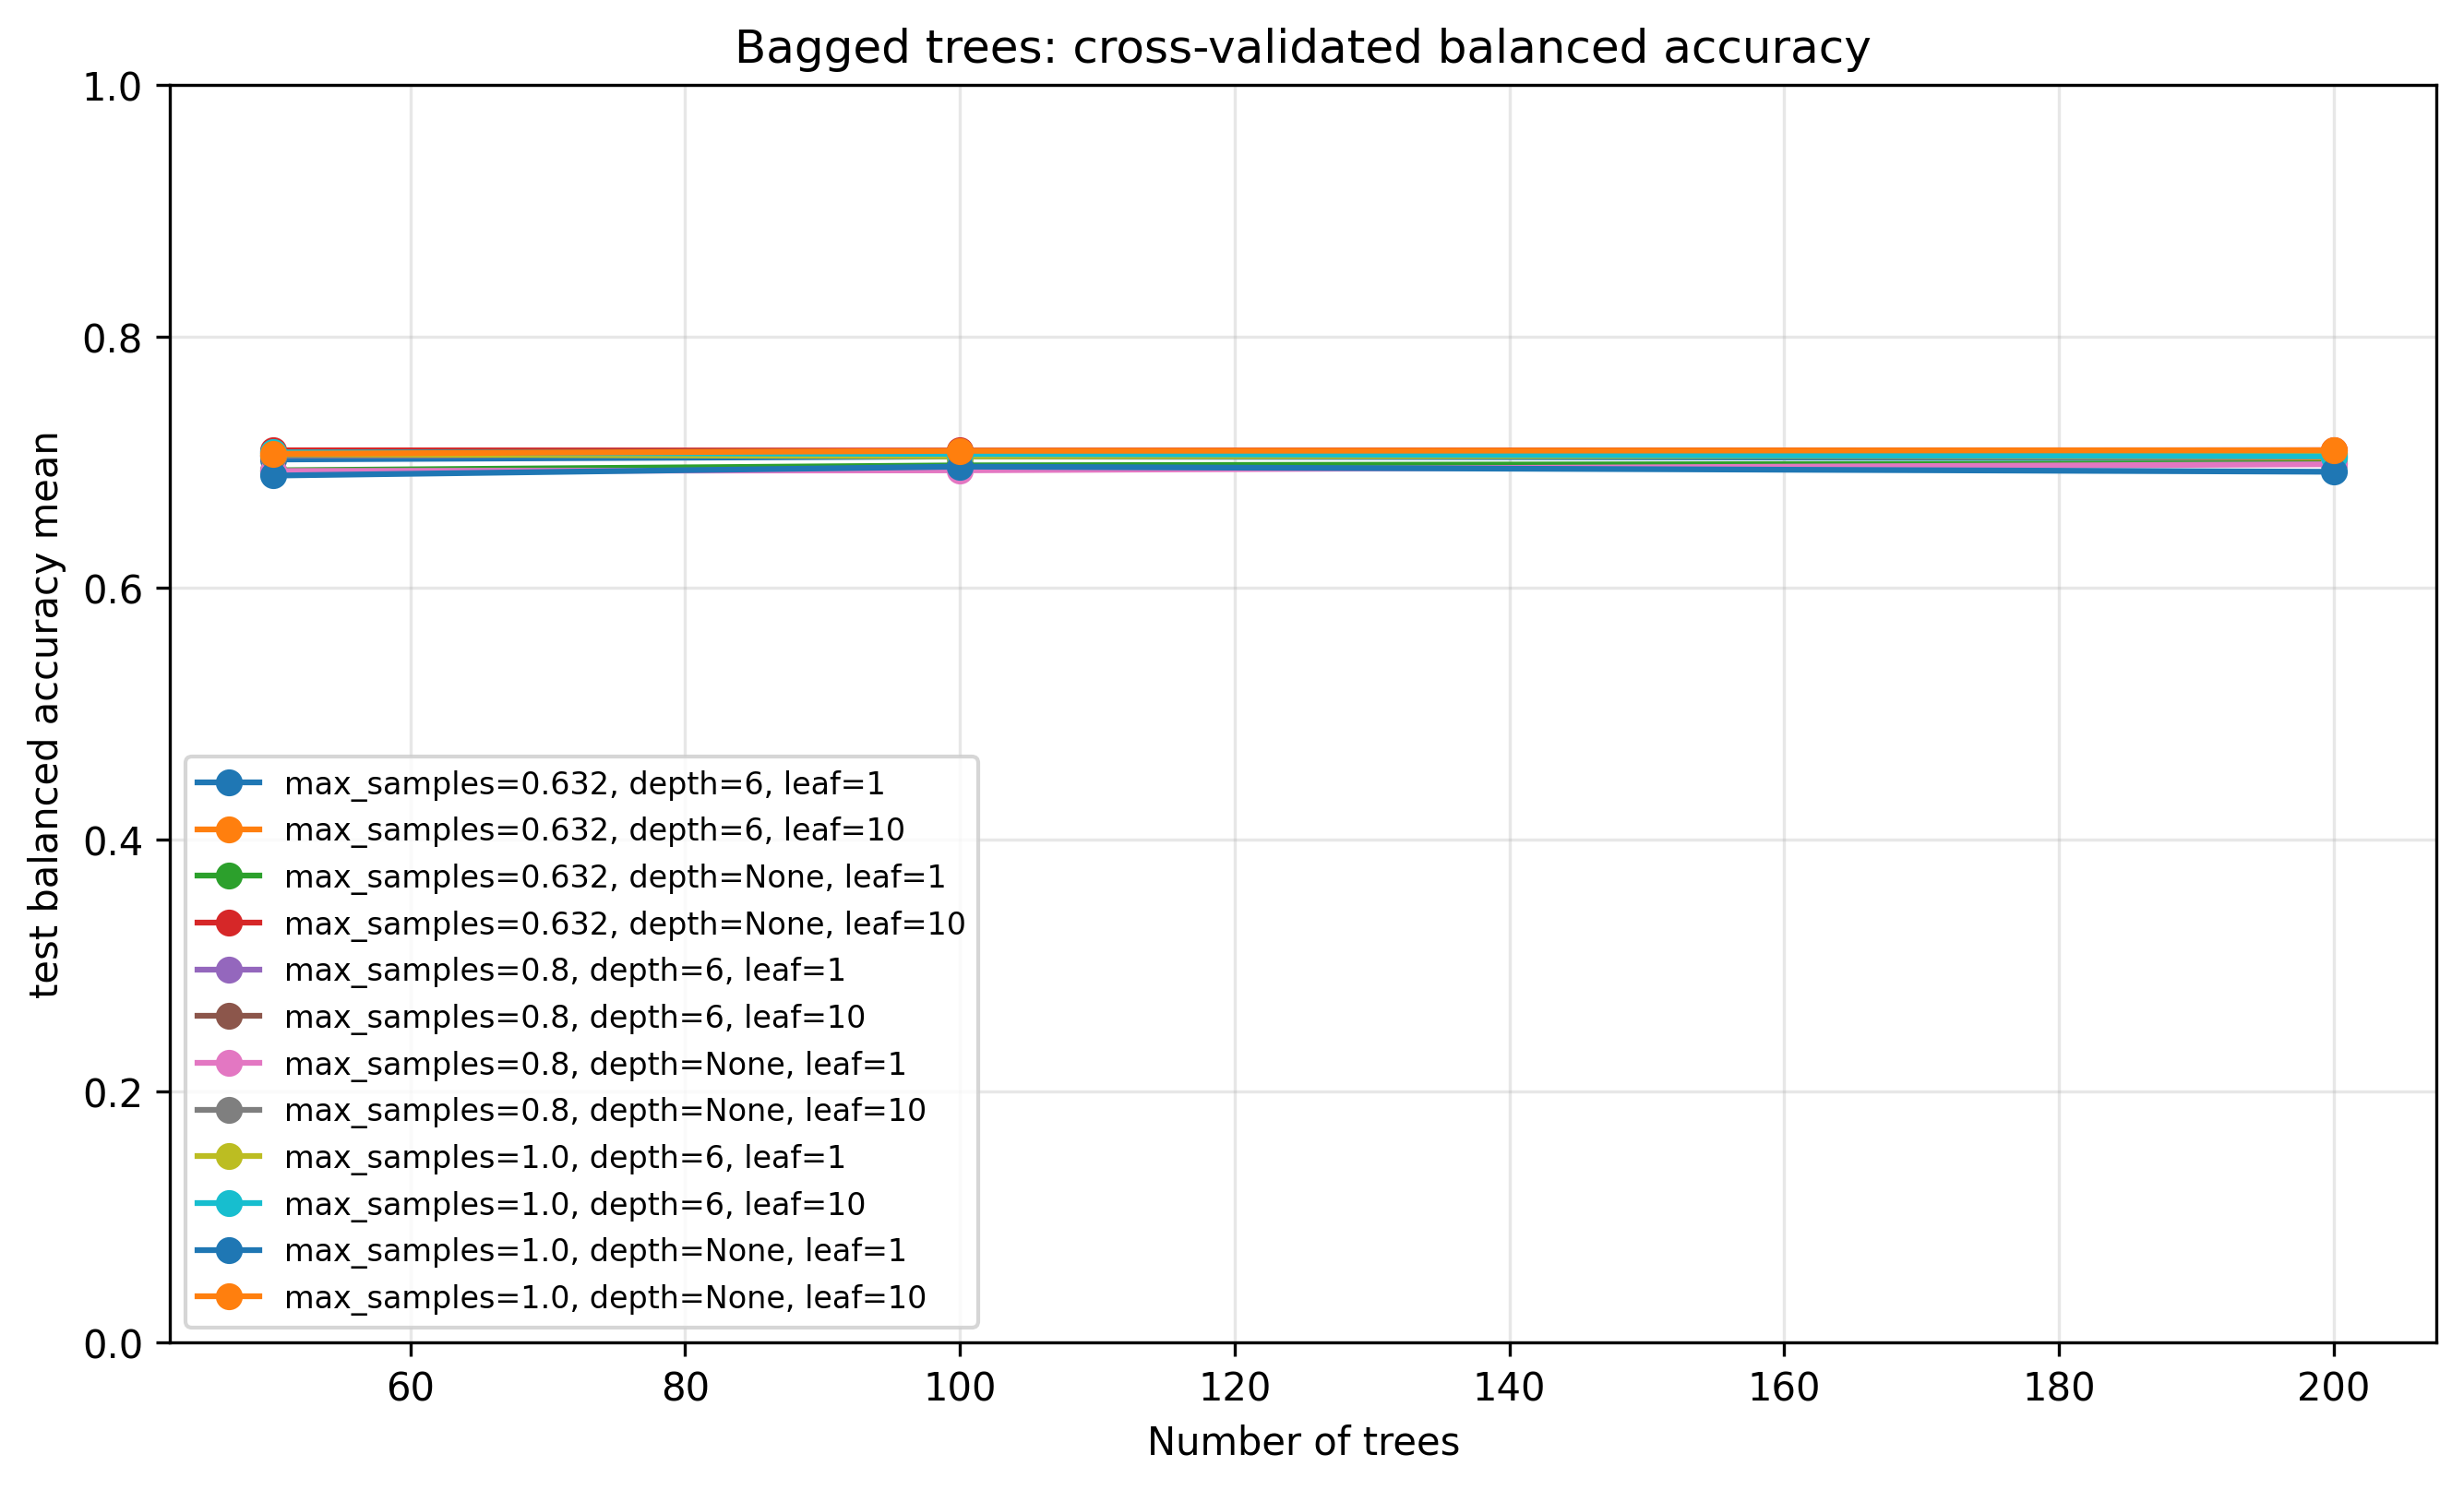
\includegraphics[width=0.88\textwidth]{../figures/bagging_balanced_accuracy_by_estimators.png}
\caption{Bagged trees: cross-validated balanced accuracy by number of trees}
\label{fig:bagging-balanced-accuracy-by-estimators}
\end{figure}

\subsection{Random-forest grid results}

Figure~\ref{fig:random-forest-pr-auc-by-depth} shows the random-forest grid from the perspective of PR-AUC. The strongest random-forest candidate uses 200 trees, maximum depth 10, \(\texttt{min\_samples\_leaf}=10\), and \(\texttt{max\_features}=\texttt{sqrt}\). Its grid-level mean PR-AUC is approximately \(0.664\).

\begin{figure}[H]
\centering
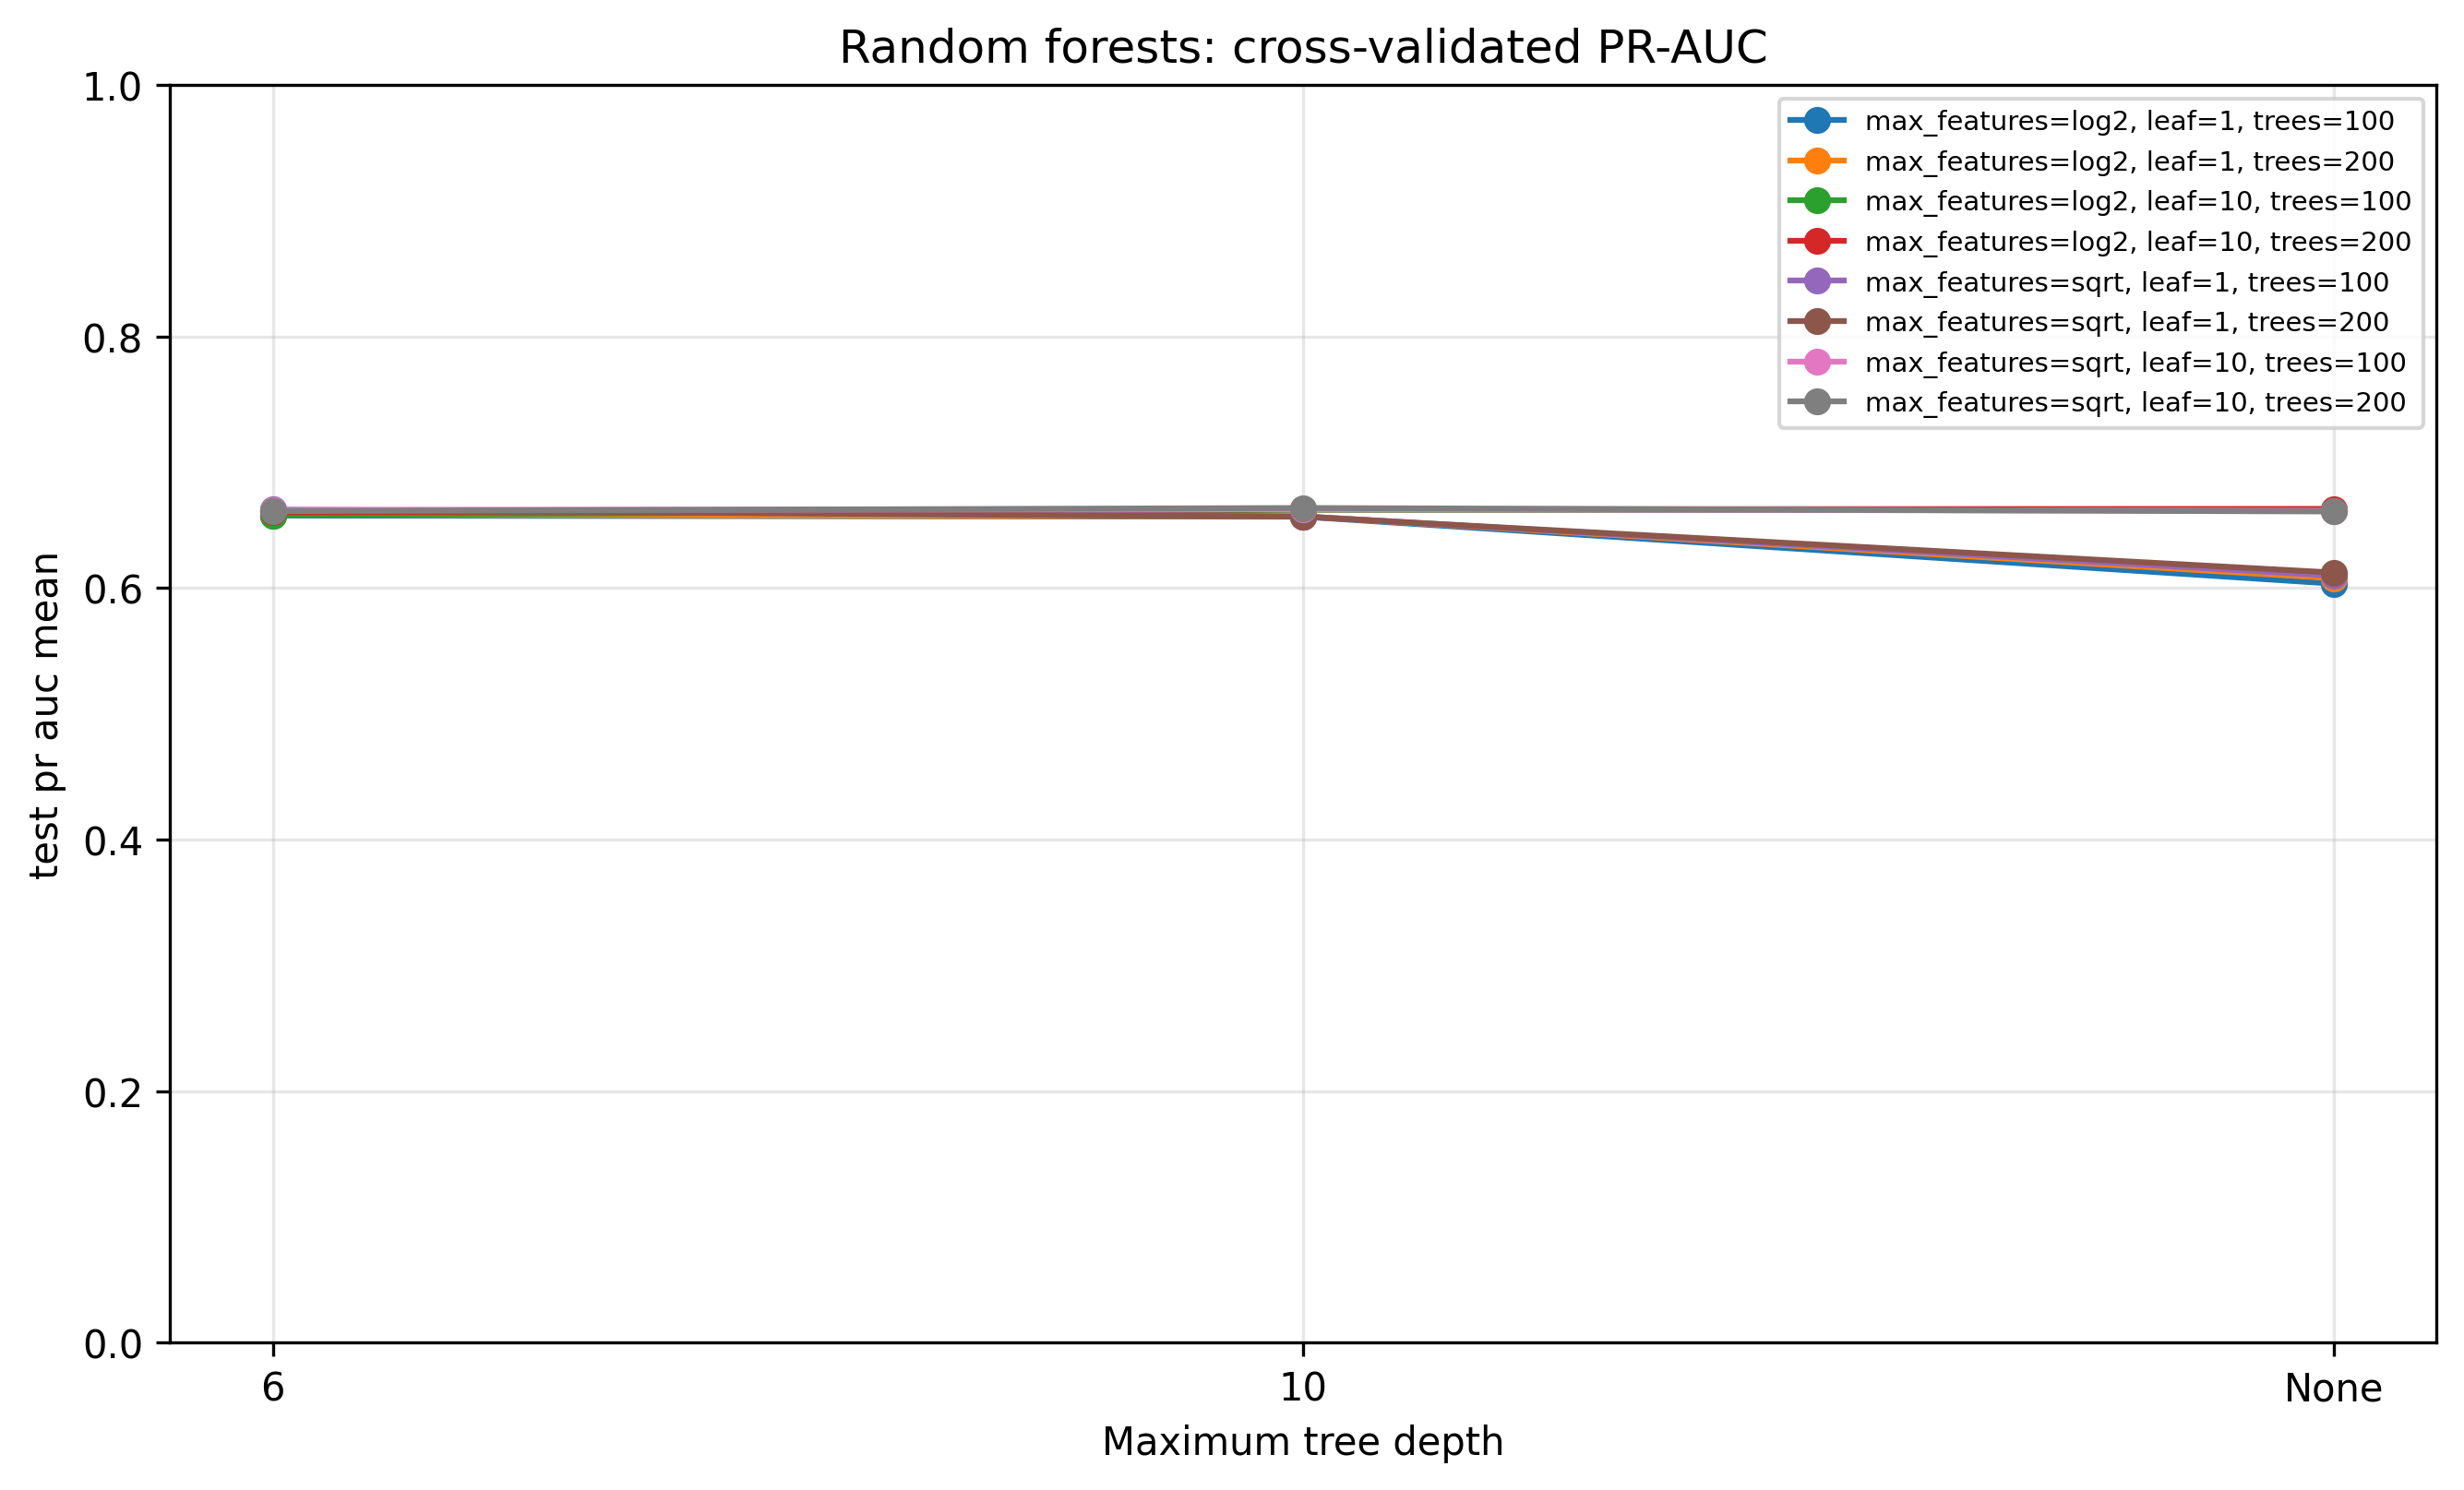
\includegraphics[width=0.88\textwidth]{../figures/random_forest_pr_auc_by_depth.png}
\caption{Random forests: cross-validated PR-AUC by maximum tree depth}
\label{fig:random-forest-pr-auc-by-depth}
\end{figure}

The unrestricted-depth random-forest settings are weaker by PR-AUC than the depth-6 and depth-10 settings. This is consistent with the general tree-regularization pattern already seen in Section~\ref{sec:decision-trees}: even inside an ensemble, overly flexible trees can add noisy splits that do not improve validation ranking performance.

Figure~\ref{fig:random-forest-balanced-accuracy-by-depth} shows the random-forest grid using balanced accuracy. The metric is again very stable across many configurations. The depth-10 settings are slightly stronger than depth 6 and unrestricted depth, but the differences are small.

\begin{figure}[H]
\centering
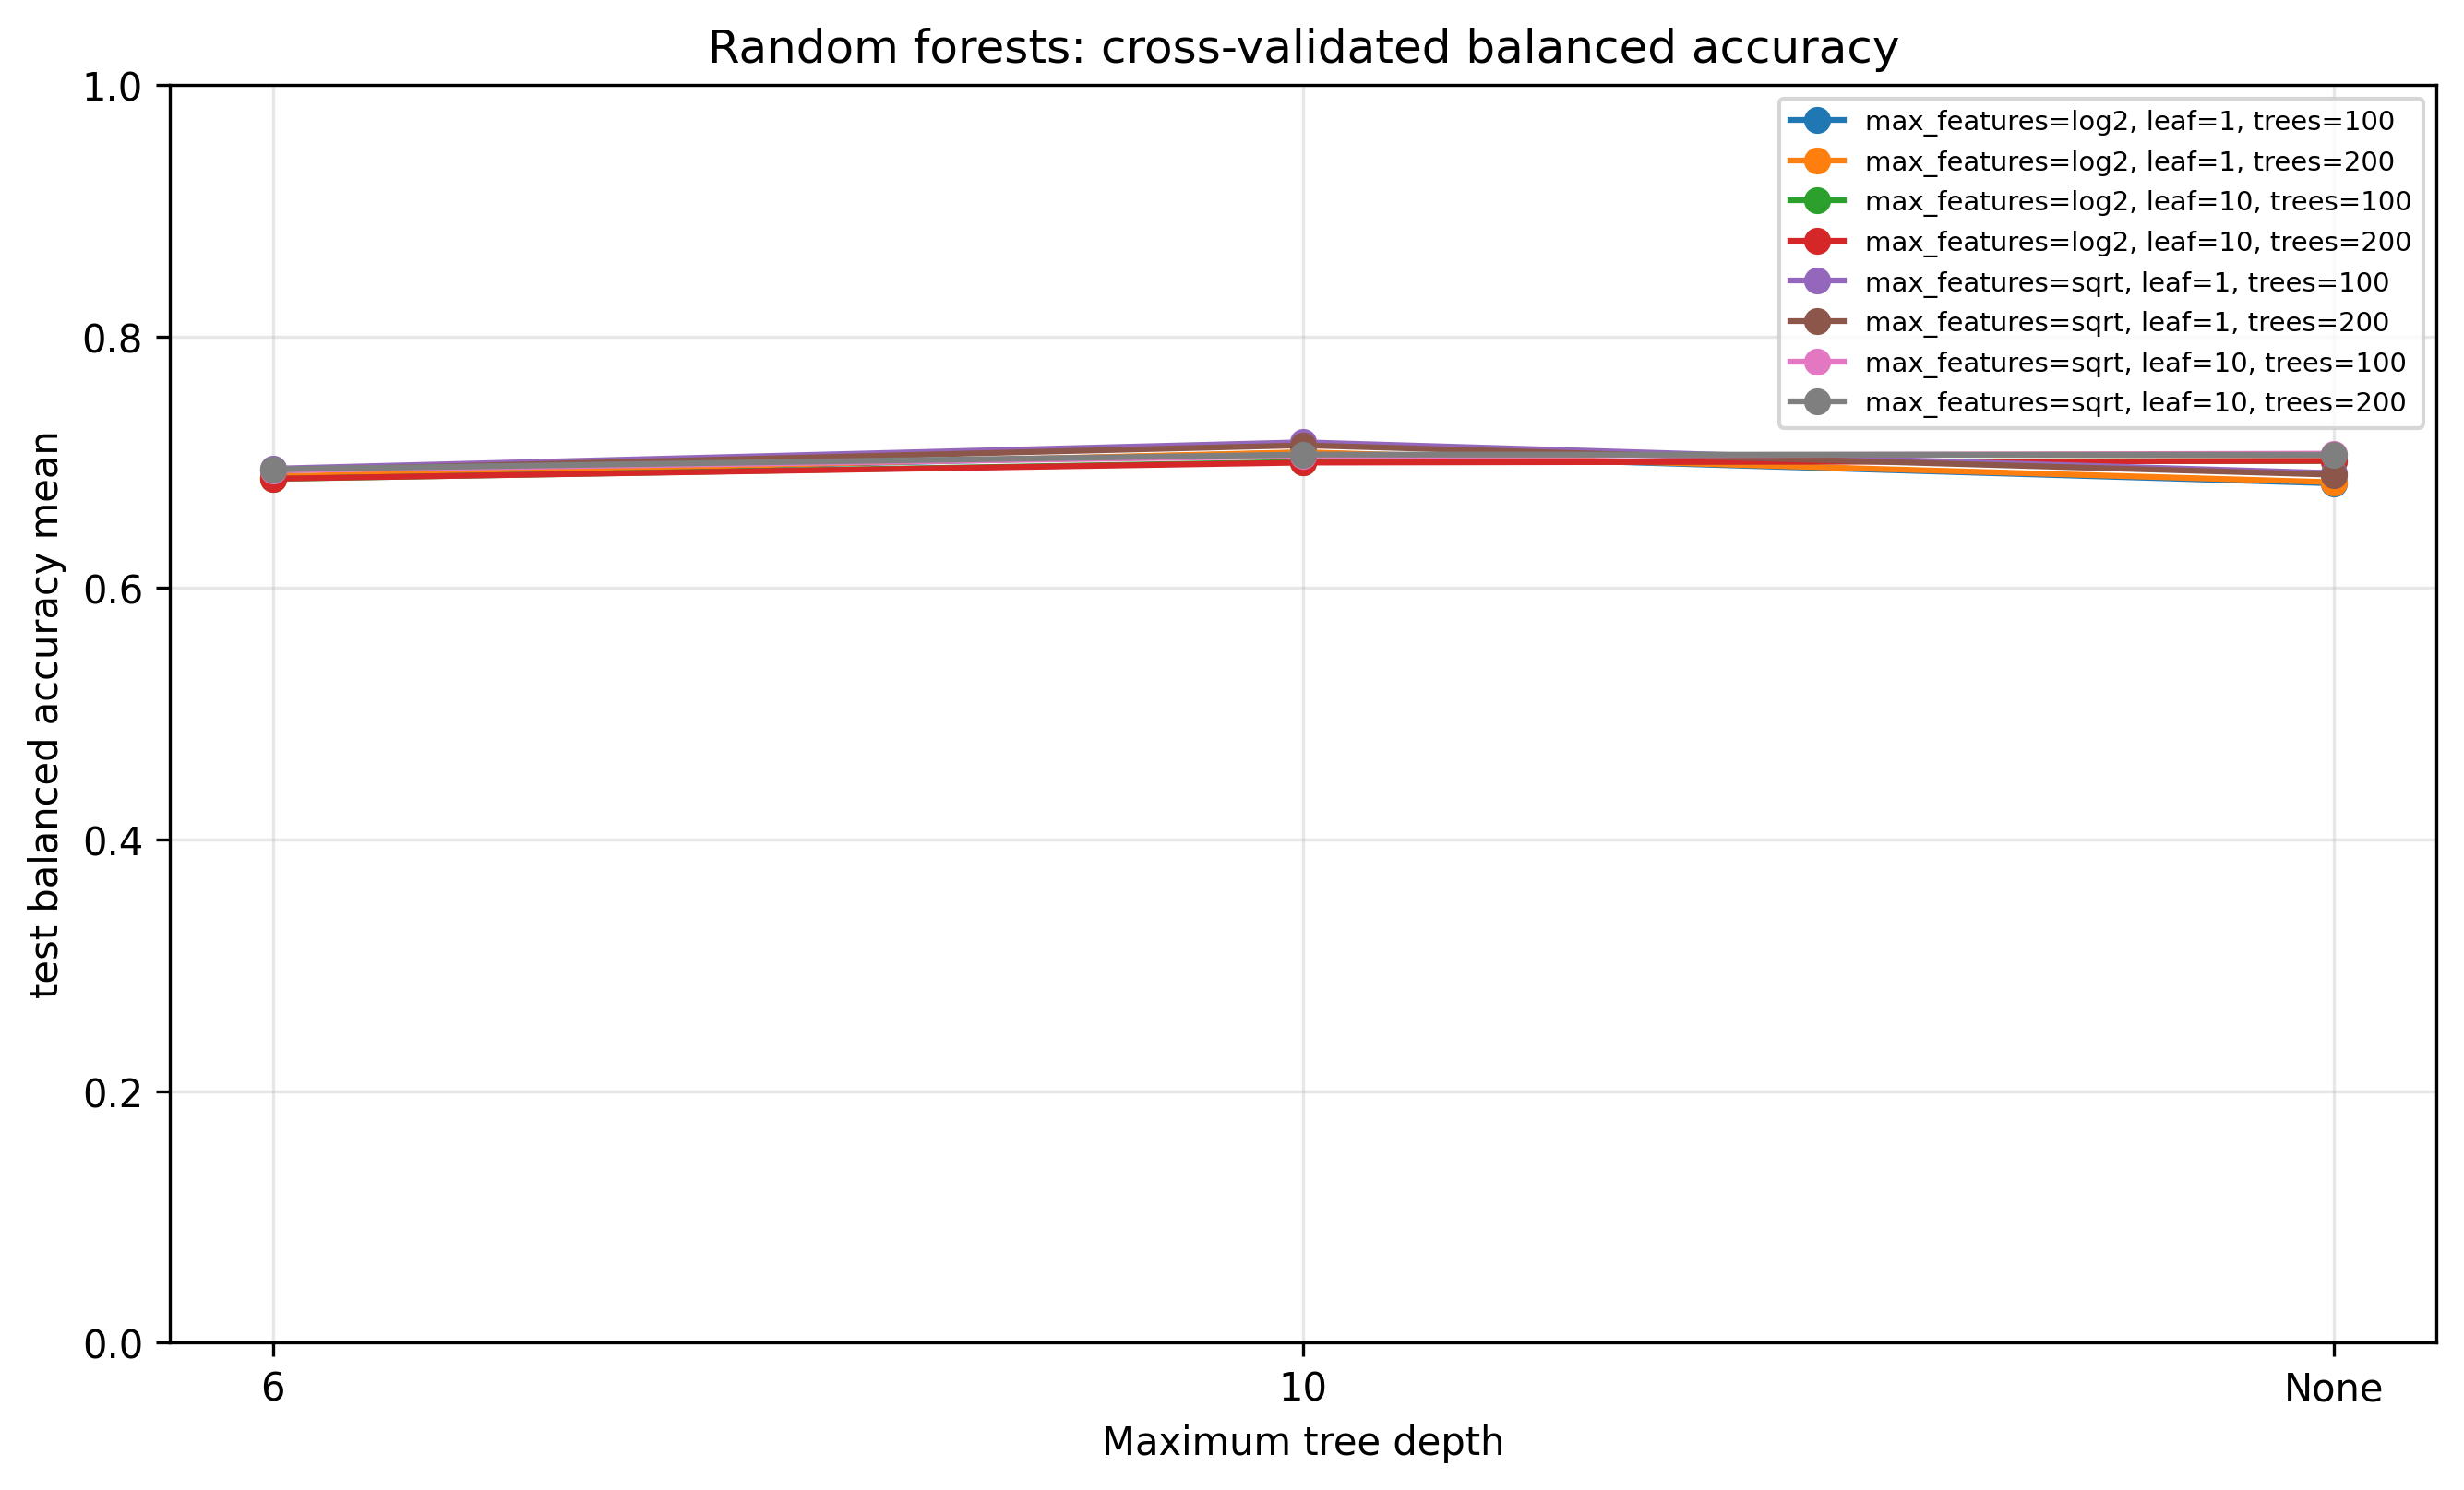
\includegraphics[width=0.88\textwidth]{../figures/random_forest_balanced_accuracy_by_depth.png}
\caption{Random forests: cross-validated balanced accuracy by maximum tree depth}
\label{fig:random-forest-balanced-accuracy-by-depth}
\end{figure}

\subsection{Model comparison}

Table~\ref{tab:bagging-random-forest-model-comparison} compares the selected tree-ensemble candidates with the selected single decision tree and a default random forest. The selected bagged-tree ensemble improves PR-AUC from approximately \(0.628\) for the single tree to approximately \(0.662\). The selected random forest obtains PR-AUC approximately \(0.660\). Both ensembles also improve ROC-AUC from approximately \(0.824\) to approximately \(0.846\) or \(0.847\).

\begin{table}[H]
\centering
\small
\resizebox{\textwidth}{!}{
\begin{tabular}{lrrrrrrrr}
\toprule
Model & Accuracy & Bal. Acc. & Precision & Recall & Specificity & \(F_1\) & ROC-AUC & PR-AUC \\
\midrule
Best bagged trees & 0.800 & 0.705 & 0.662 & 0.504 & 0.907 & 0.572 & 0.846 & 0.662 \\
Best random forest & 0.804 & 0.706 & 0.678 & 0.498 & 0.914 & 0.574 & 0.847 & 0.660 \\
Selected single decision tree & 0.789 & 0.701 & 0.624 & 0.514 & 0.888 & 0.564 & 0.824 & 0.628 \\
Default random forest, 100 estimators & 0.788 & 0.691 & 0.629 & 0.486 & 0.896 & 0.548 & 0.821 & 0.608 \\
\bottomrule
\end{tabular}
}
\caption{Cross-validated bagging and random-forest model comparison on the training set}
\label{tab:bagging-random-forest-model-comparison}
\end{table}

The main conclusion is not that plain bagging is statistically superior to random forests. The two selected ensemble variants are very close. Plain bagging has the slightly higher PR-AUC point estimate, while the random forest has slightly higher ROC-AUC, balanced accuracy, precision, specificity, and \(F_1\). These differences are too small to interpret as statistical evidence that one tree-ensemble variant is truly better. The stronger conclusion is that bagging-based ensembles clearly improve over the single decision tree.

The corresponding positive-first confusion-matrix counts are shown in Table~\ref{tab:bagging-random-forest-confusion}. At the default threshold, the selected bagged trees detect \(753\) of the \(1495\) churners and produce \(385\) false positives. The selected random forest detects \(744\) churners and produces \(354\) false positives. Thus, the selected random forest is slightly more conservative at the default threshold, with fewer positives flagged overall.

\begin{table}[H]
\centering
\small
\begin{tabular}{lrrrrr}
\toprule
Model & TP & FN & FP & TN & Pred. positive rate \\
\midrule
Best bagged trees & 753 & 742 & 385 & 3754 & 0.202 \\
Best random forest & 744 & 751 & 354 & 3785 & 0.195 \\
Selected single decision tree & 769 & 726 & 463 & 3676 & 0.219 \\
Default random forest, 100 estimators & 727 & 768 & 429 & 3710 & 0.205 \\
\bottomrule
\end{tabular}
\caption{Positive-first confusion-matrix counts for bagging and random forests}
\label{tab:bagging-random-forest-confusion}
\end{table}

\subsection{Out-of-bag diagnostics}

Table~\ref{tab:bagging-random-forest-oob} reports out-of-bag diagnostics for the selected ensemble candidates. The out-of-bag PR-AUC values are close to the cross-validated PR-AUC values, which is reassuring. The selected bagged-tree ensemble has out-of-bag PR-AUC approximately \(0.660\), while the selected random forest has out-of-bag PR-AUC approximately \(0.663\).

\begin{table}[H]
\centering
\small
\begin{tabular}{lrrrr}
\toprule
Model & OOB accuracy & OOB valid obs. & OOB ROC-AUC & OOB PR-AUC \\
\midrule
Best bagged trees & 0.801 & 5634 & 0.845 & 0.660 \\
Best random forest & 0.802 & 5634 & 0.847 & 0.663 \\
\bottomrule
\end{tabular}
\caption{Out-of-bag diagnostics for selected bagging-based ensembles}
\label{tab:bagging-random-forest-oob}
\end{table}

These out-of-bag diagnostics support the earlier caution about the bagging versus random-forest comparison. The fixed-grid CV PR-AUC point estimate is slightly higher for plain bagging, while the out-of-bag PR-AUC is slightly higher for the random forest. This does not create a contradiction. It shows that the two ensemble variants are close enough that small changes in evaluation procedure can change their ordering.

\subsection{Threshold behaviour}

Figure~\ref{fig:bagging-random-forest-threshold-tradeoff} shows the threshold tradeoff for the selected PR-AUC representative, the bagged-tree ensemble. Lower thresholds increase recall but reduce precision and specificity. Higher thresholds reduce the number of flagged customers, raising precision and specificity but lowering recall.

\begin{figure}[H]
\centering
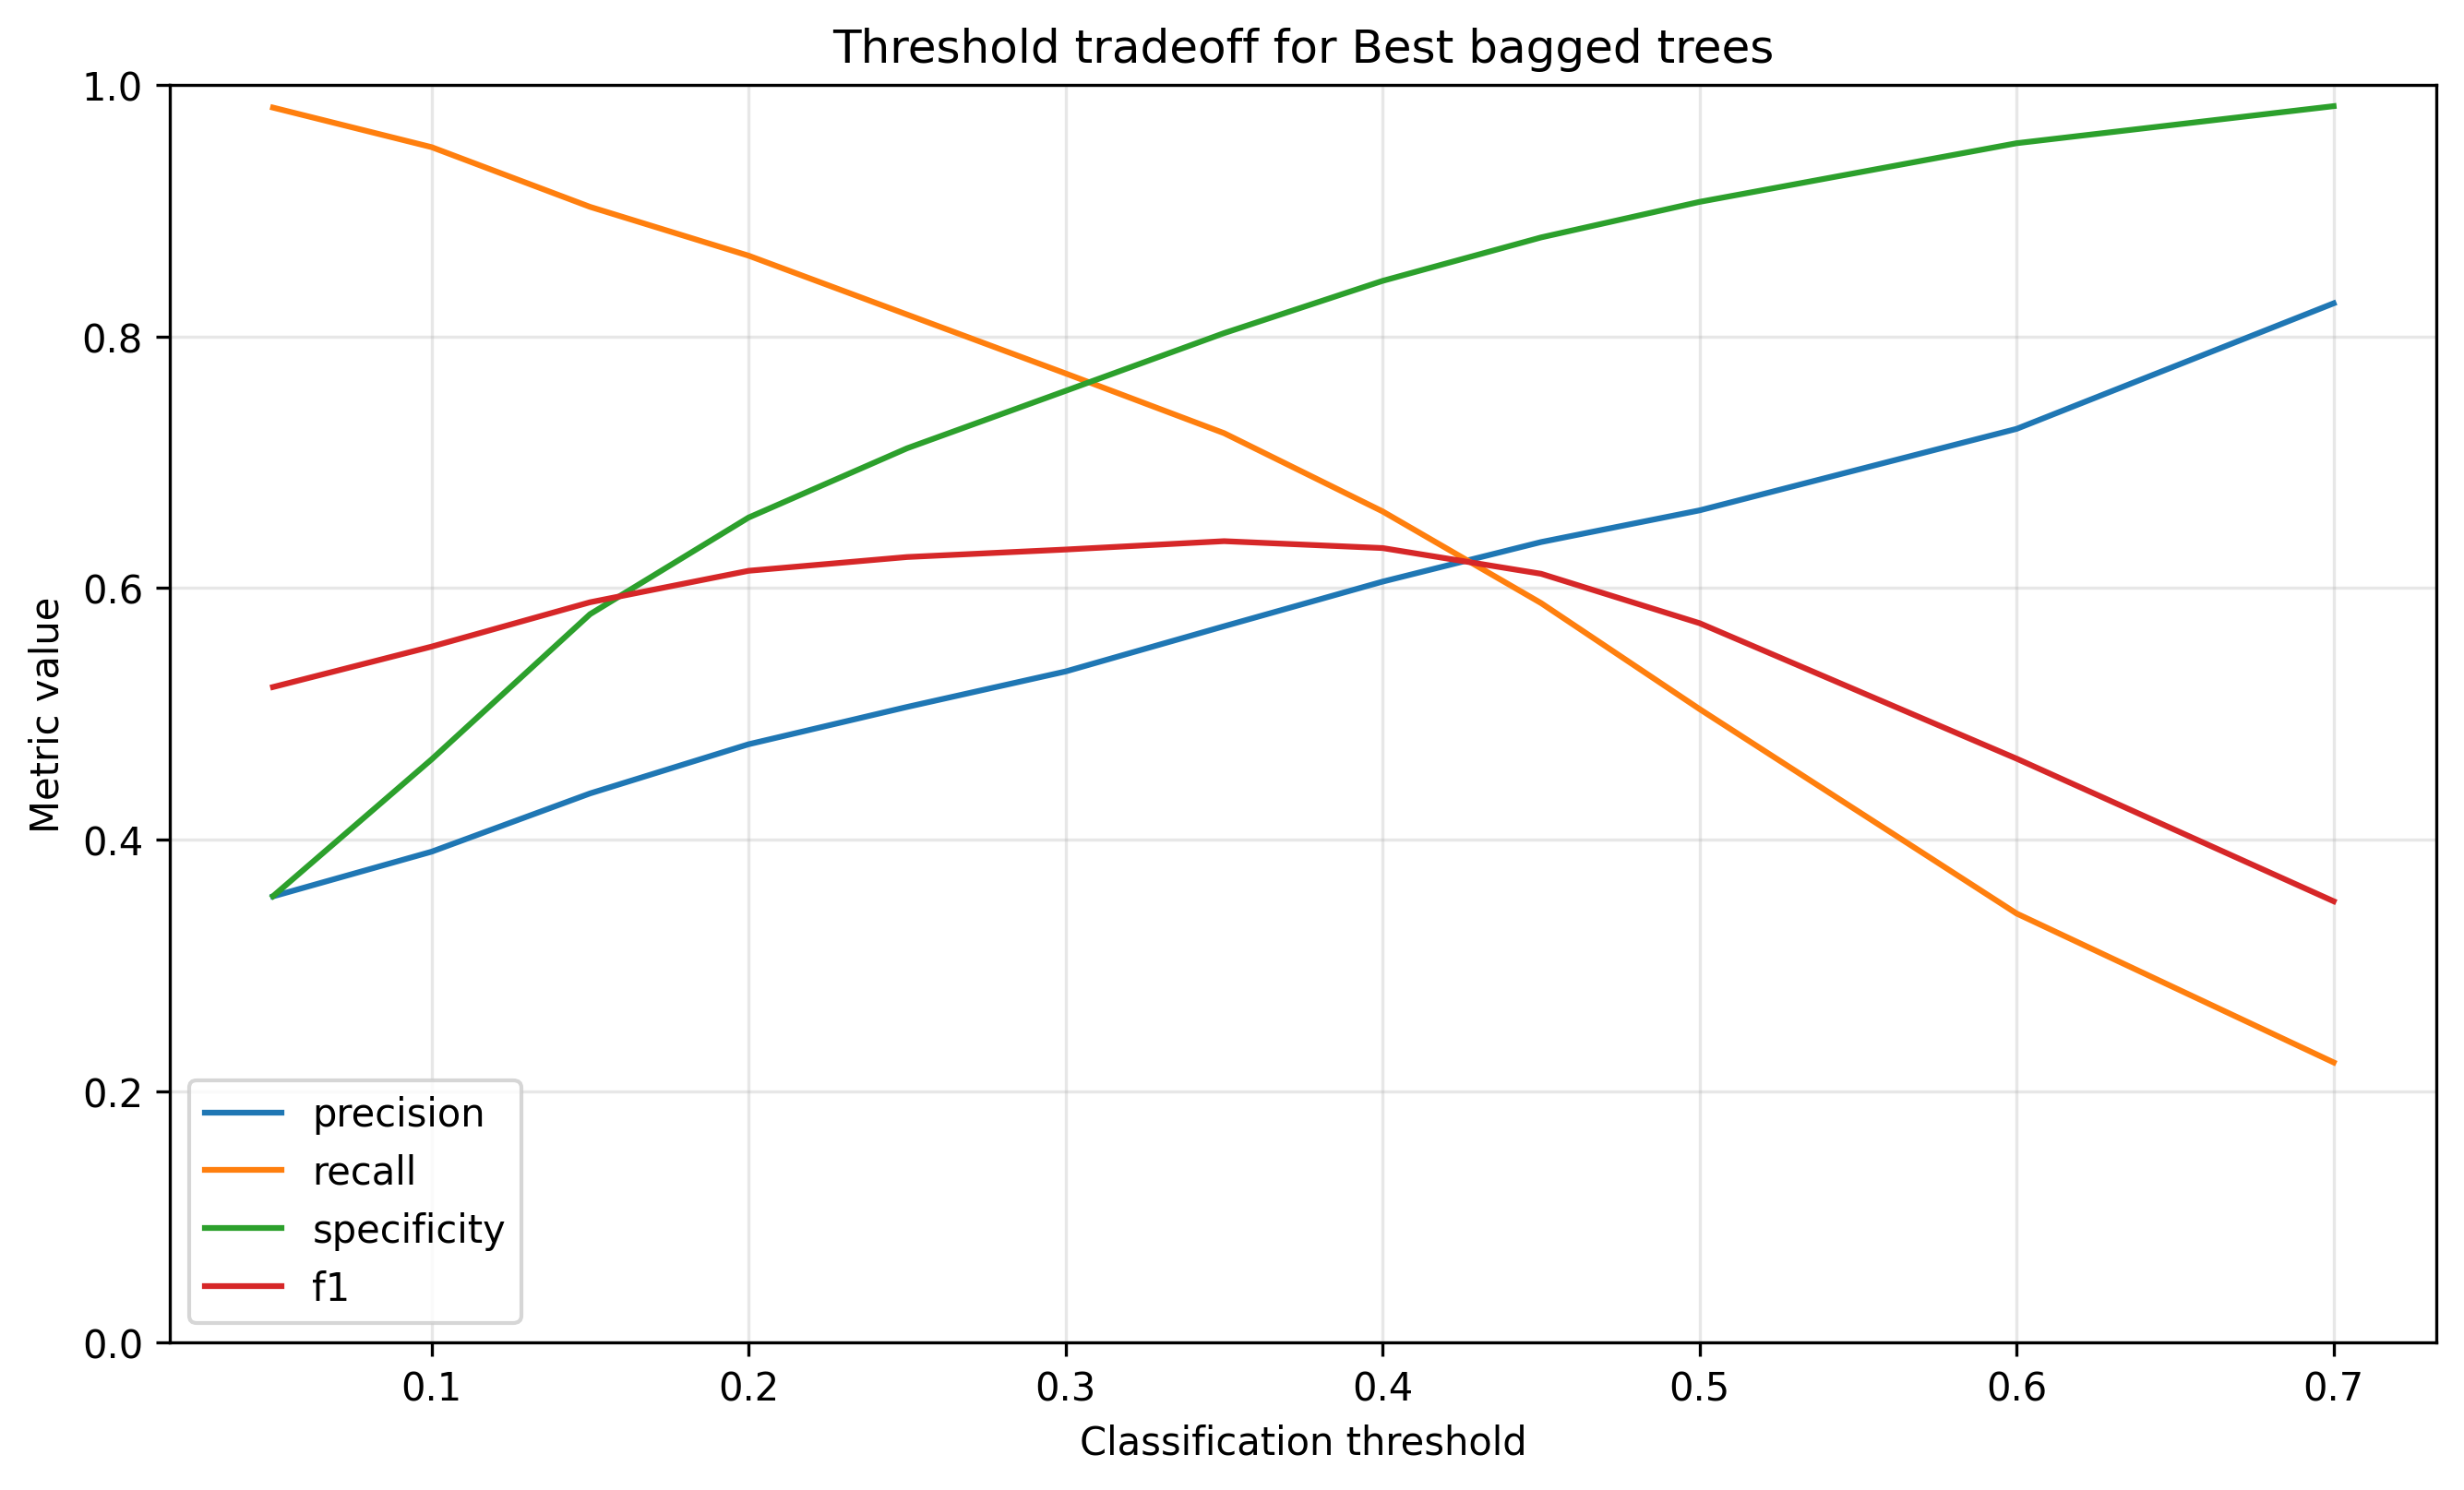
\includegraphics[width=0.88\textwidth]{../figures/bagging_random_forest_threshold_tradeoff.png}
\caption{Threshold tradeoff for the selected bagged-tree ensemble}
\label{fig:bagging-random-forest-threshold-tradeoff}
\end{figure}

At threshold \(0.30\), the selected bagged trees have recall approximately \(0.772\), precision approximately \(0.531\), specificity approximately \(0.762\), and \(F_1\) approximately \(0.629\). At threshold \(0.40\), recall is approximately \(0.665\), precision approximately \(0.604\), specificity approximately \(0.843\), and \(F_1\) approximately \(0.633\). At the default threshold \(0.50\), recall falls to approximately \(0.504\), while precision rises to approximately \(0.662\). This again confirms that threshold choice is a separate operating decision and should not be confused with model ranking performance.

\subsection{ROC and precision-recall curves}

Figure~\ref{fig:bagging-random-forest-roc-curve} shows the ROC curve for the selected bagged-tree ensemble. The ROC-AUC is approximately \(0.846\), which improves over the selected single decision tree.

\begin{figure}[H]
\centering
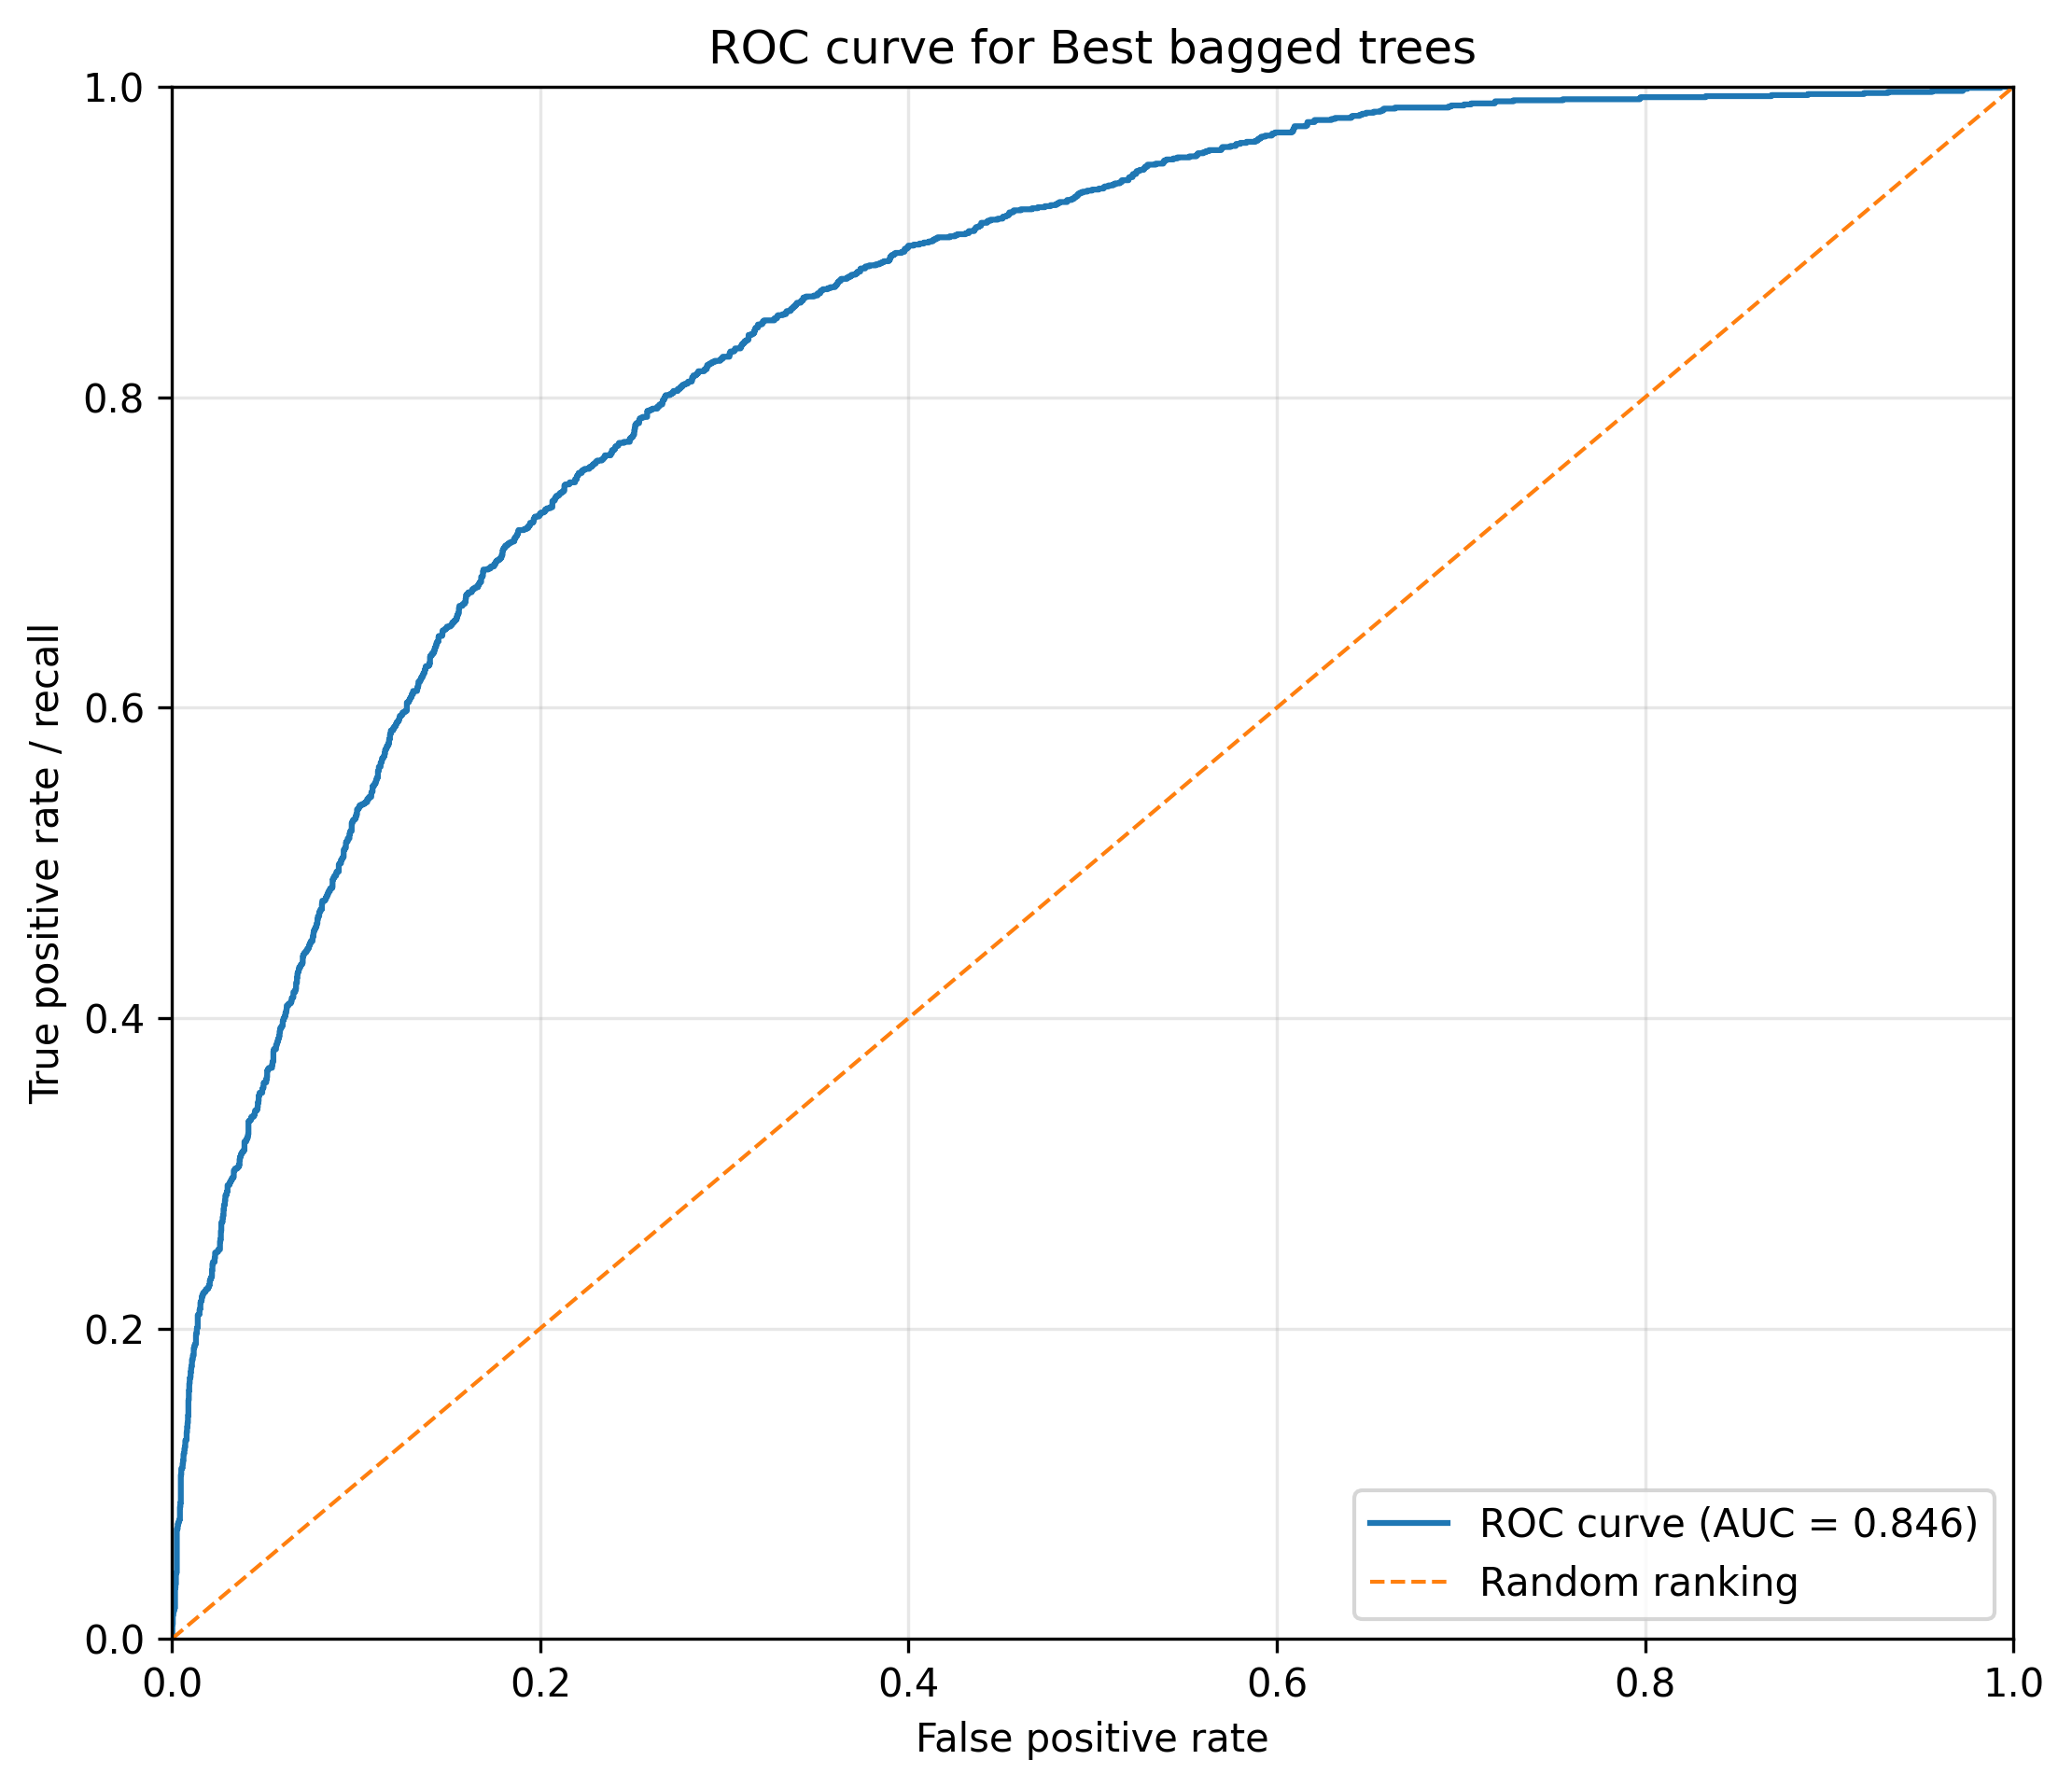
\includegraphics[width=0.88\textwidth]{../figures/bagging_random_forest_roc_curve.png}
\caption{ROC curve for the selected bagged-tree ensemble}
\label{fig:bagging-random-forest-roc-curve}
\end{figure}

Figure~\ref{fig:bagging-random-forest-pr-curve} shows the corresponding precision-recall curve. The PR-AUC is approximately \(0.661\), well above the positive-rate baseline of approximately \(0.265\). The curve shows that high precision is possible only for the highest-risk customers, while precision gradually decreases as recall approaches one.

\begin{figure}[H]
\centering
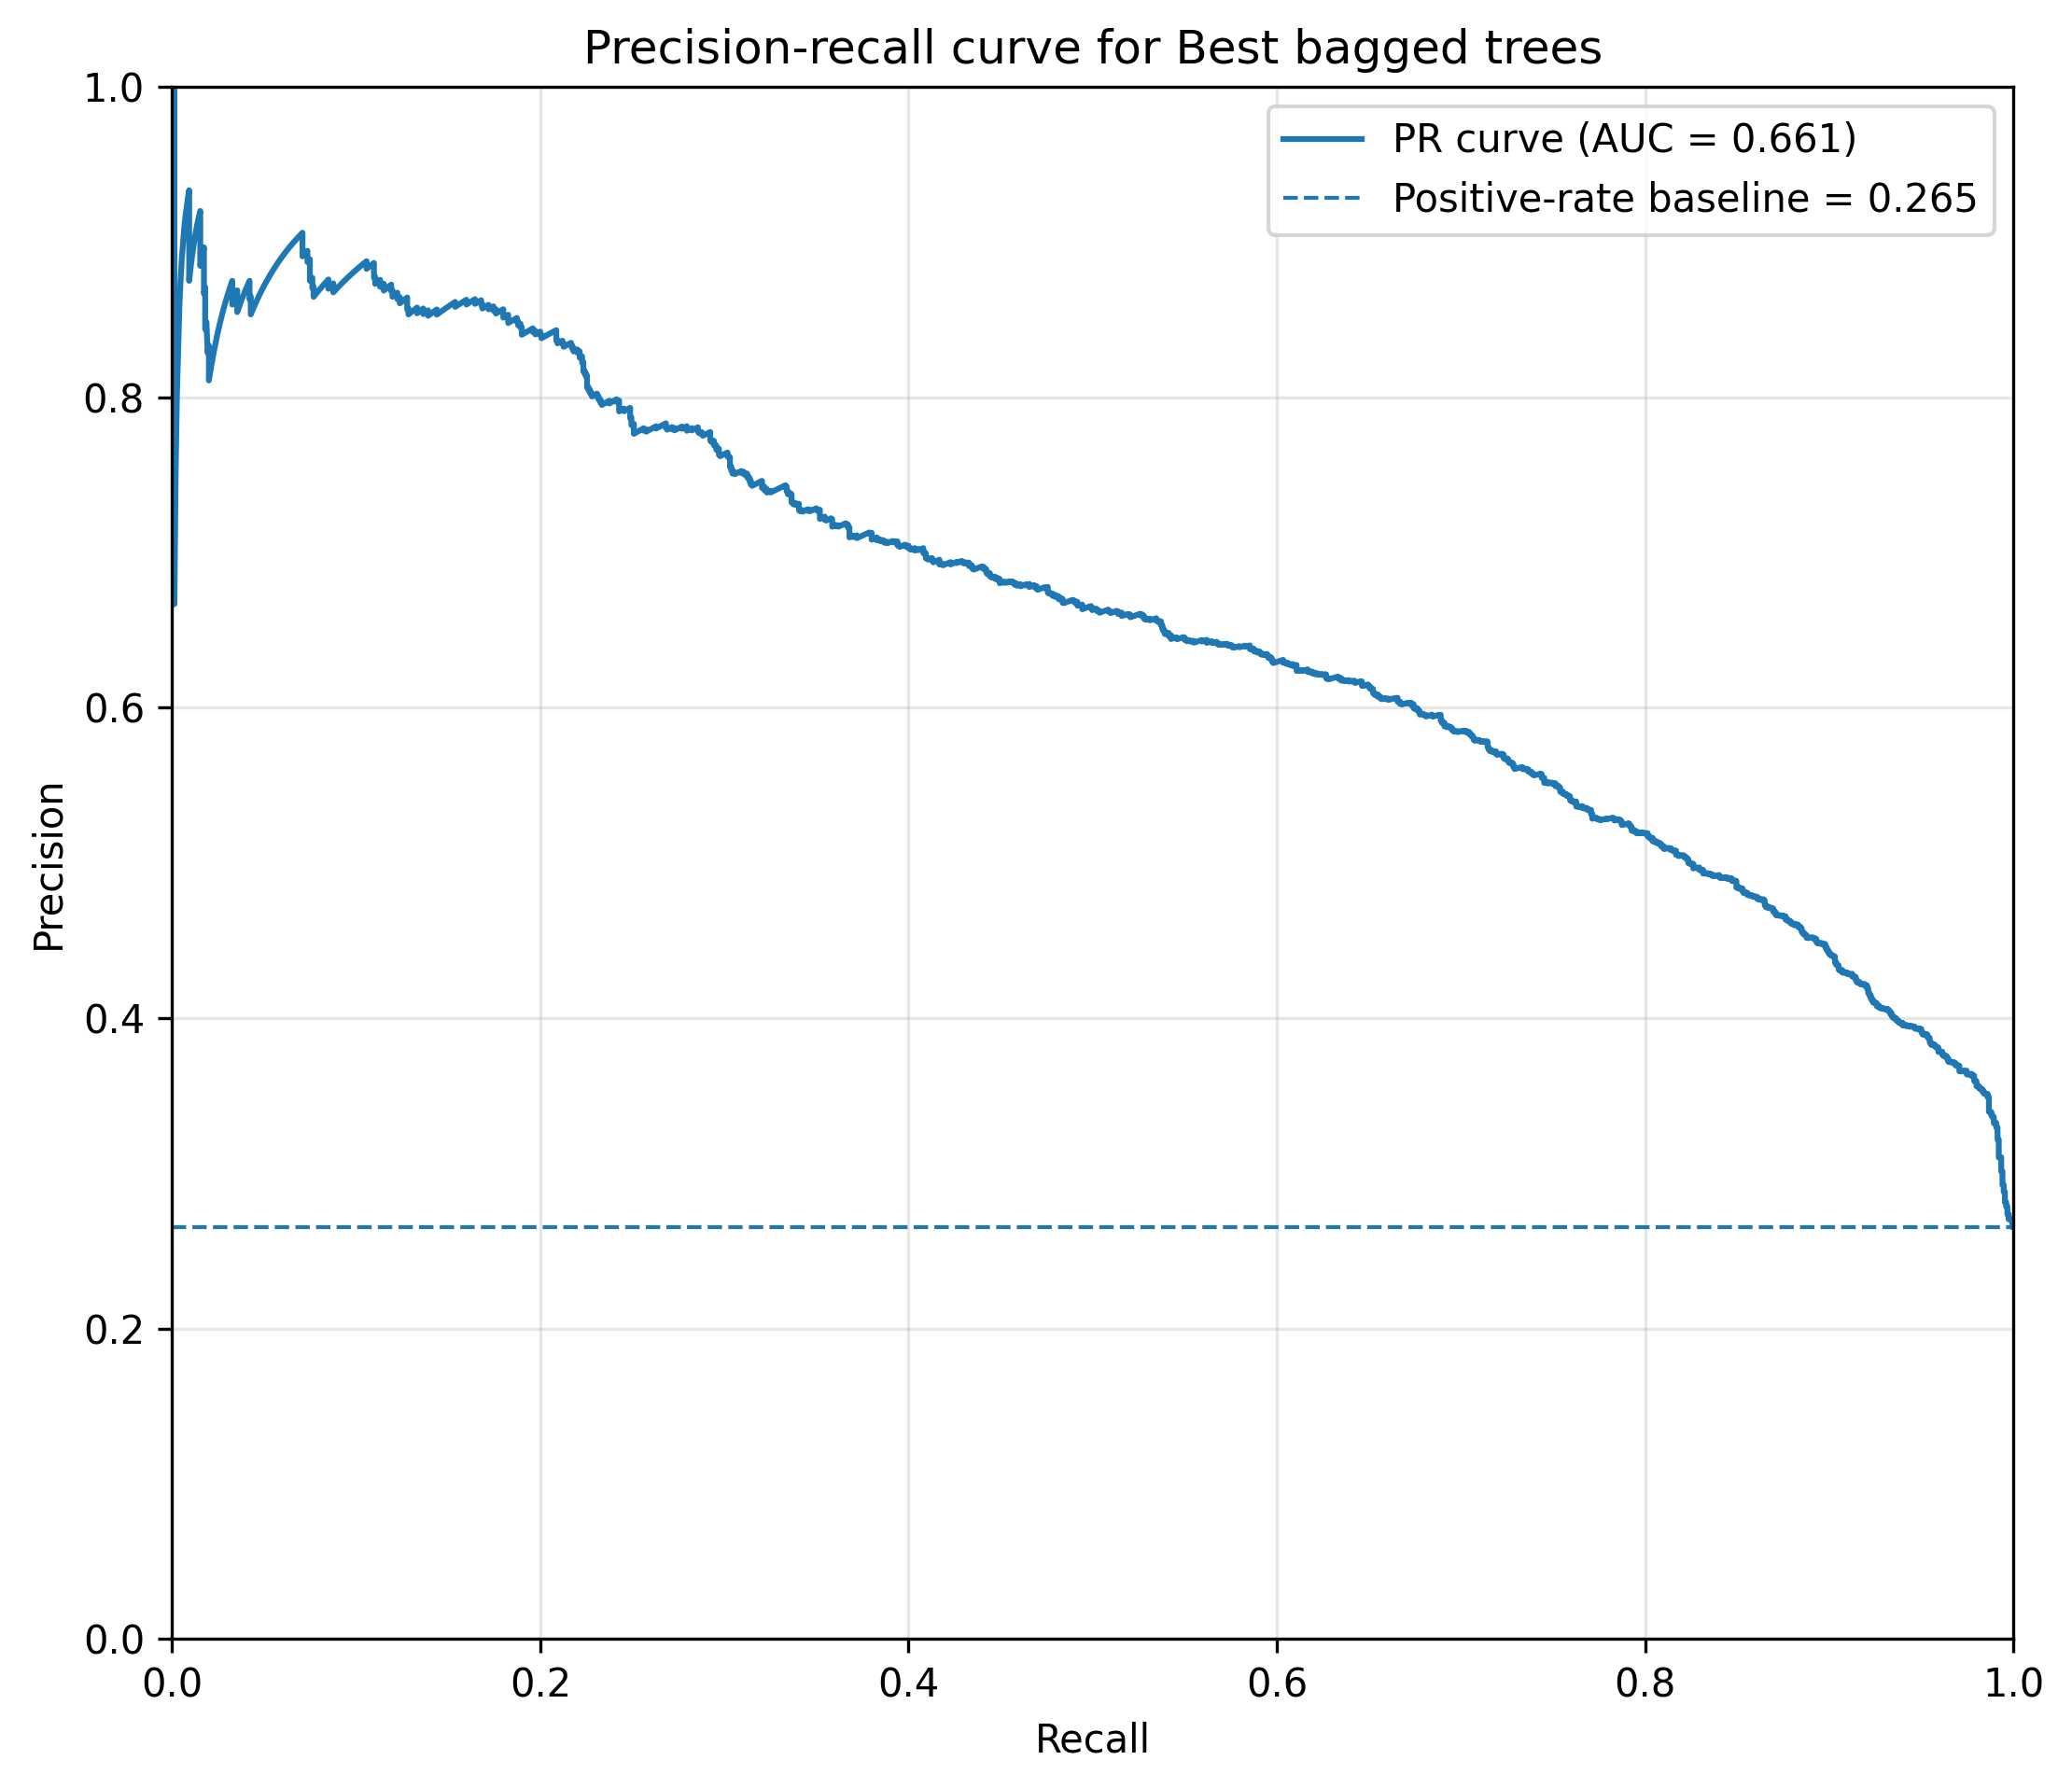
\includegraphics[width=0.88\textwidth]{../figures/bagging_random_forest_precision_recall_curve.png}
\caption{Precision-recall curve for the selected bagged-tree ensemble}
\label{fig:bagging-random-forest-pr-curve}
\end{figure}

\subsection{Random-forest feature importance}

Although the selected PR-AUC representative is the bagged-tree ensemble, the best random forest is retained as a close comparator and as a useful interpretation model. Figure~\ref{fig:random-forest-feature-importance} shows impurity-based feature importance for the best random forest.

\begin{figure}[H]
\centering
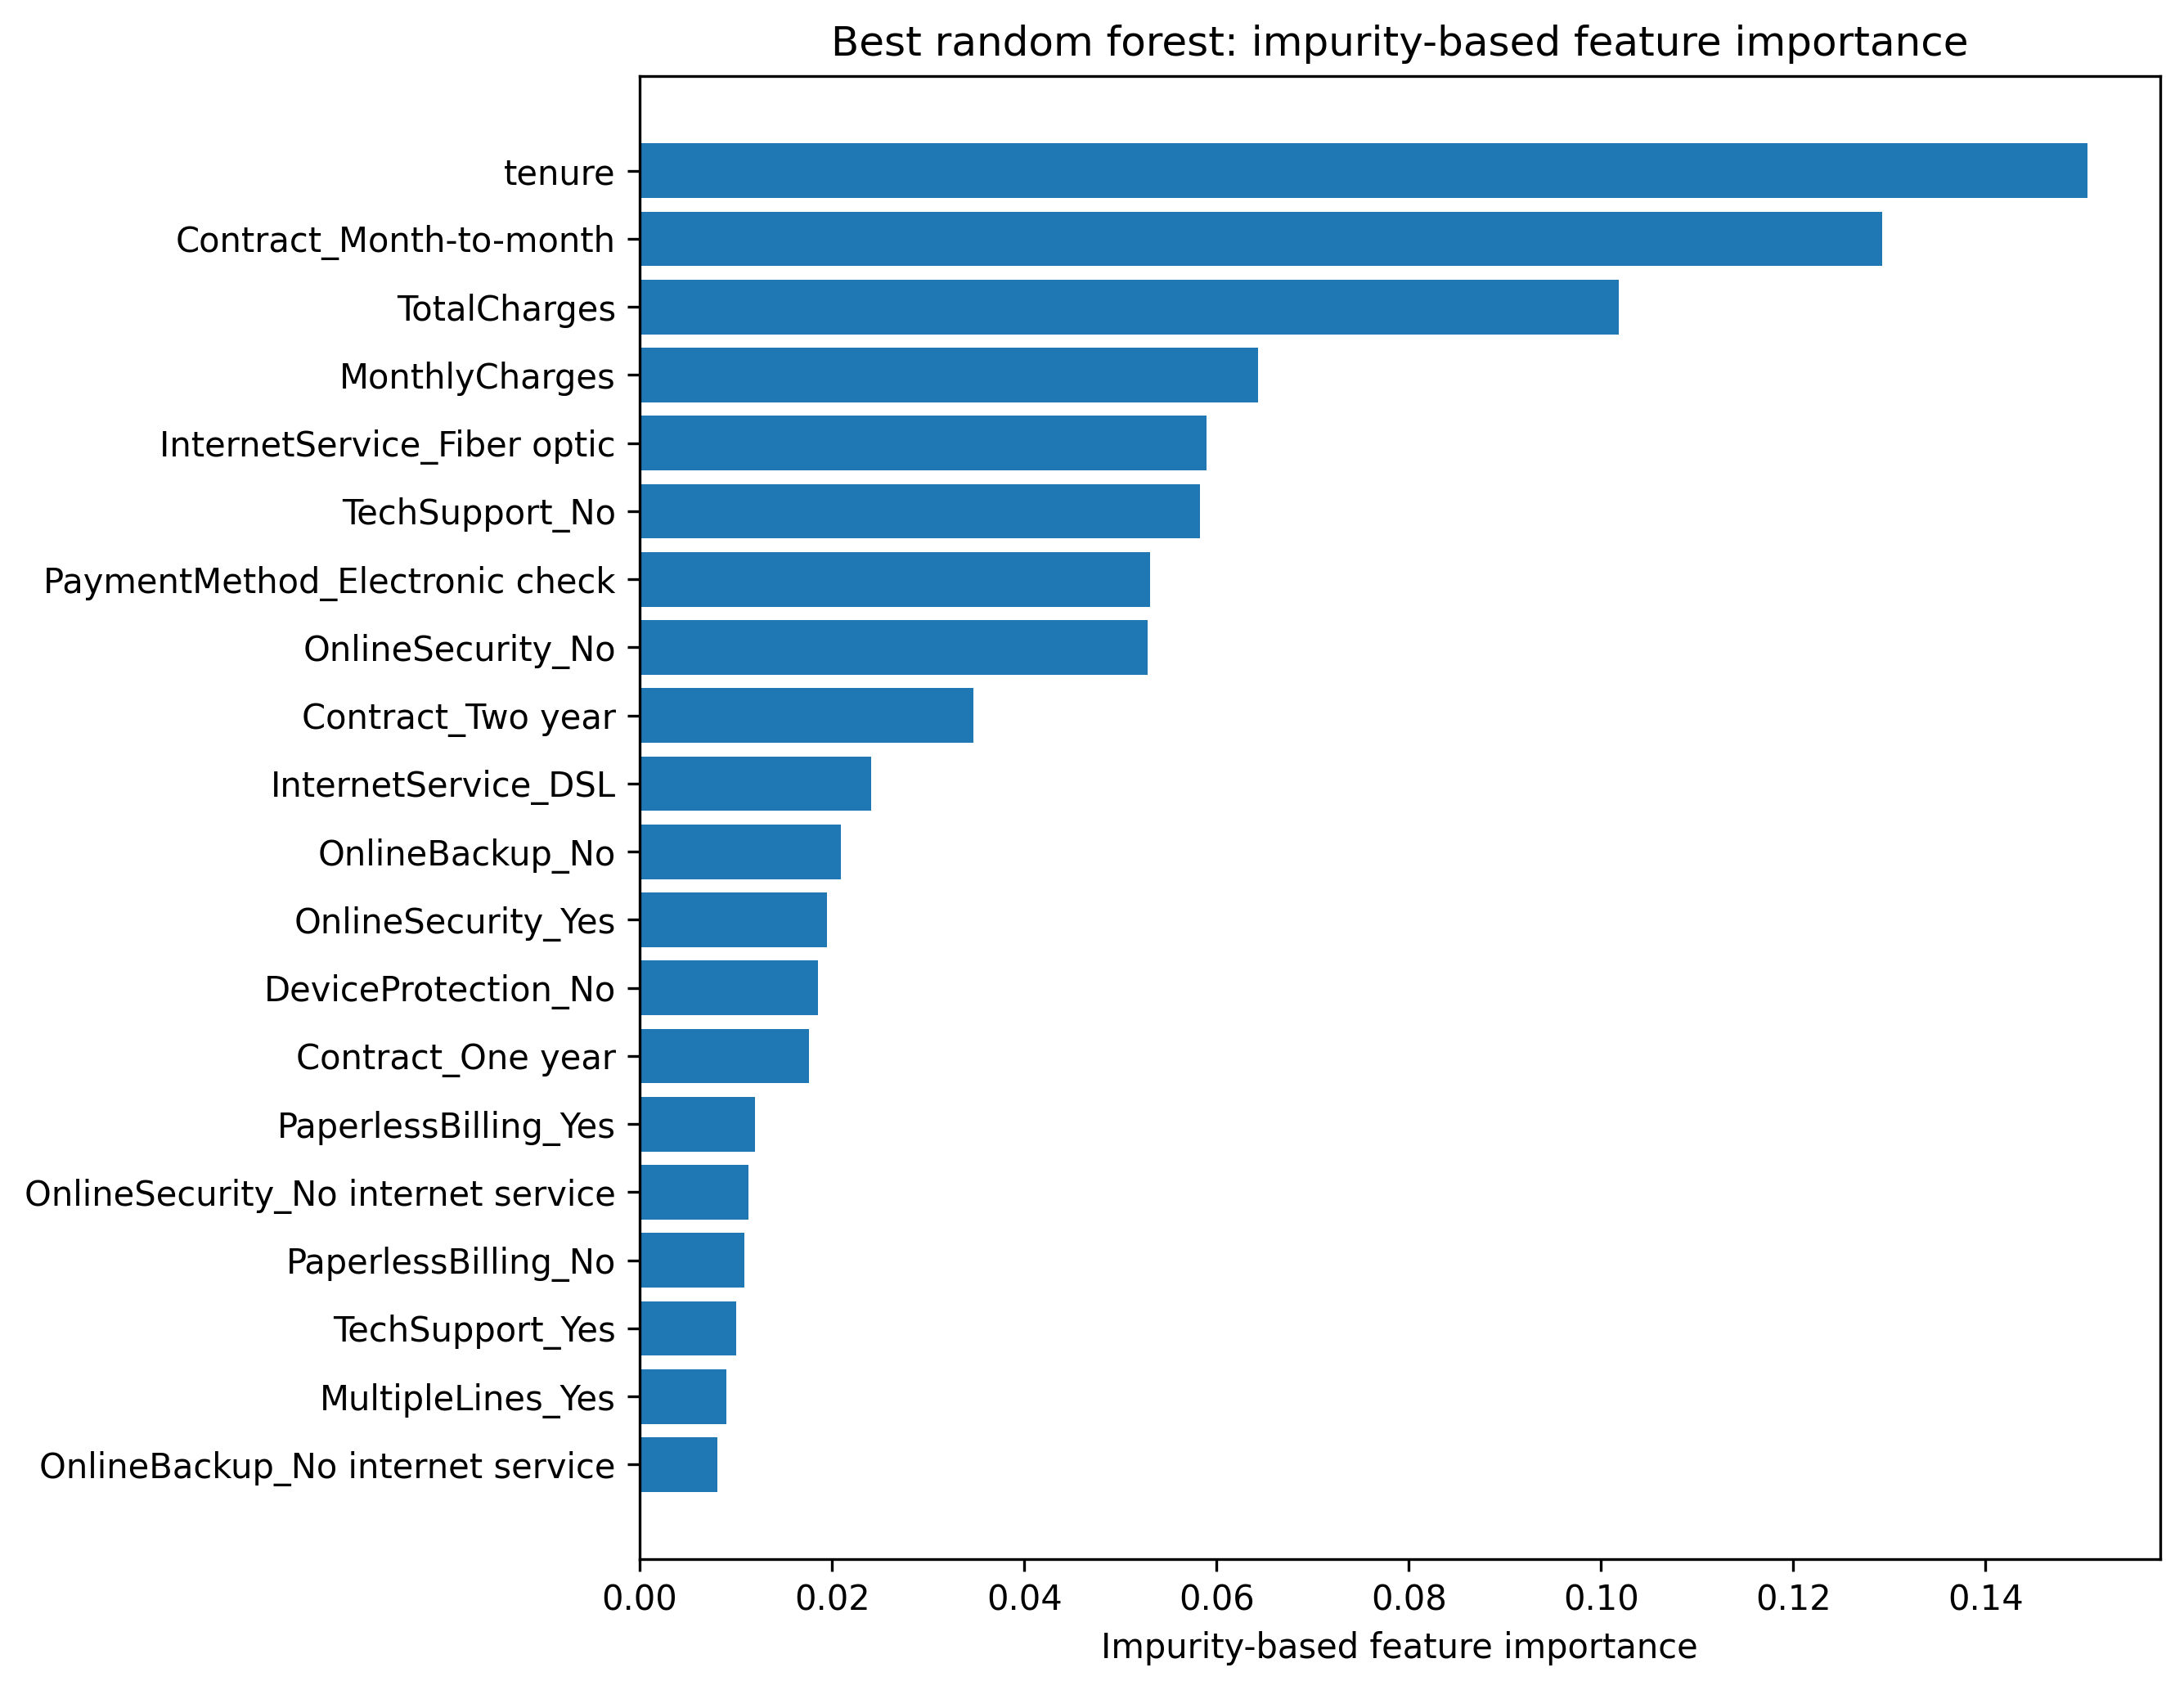
\includegraphics[width=0.88\textwidth]{../figures/random_forest_feature_importance.png}
\caption{Best random forest: impurity-based feature importance}
\label{fig:random-forest-feature-importance}
\end{figure}

The most important variables are tenure, month-to-month contract status, total charges, monthly charges, fibre-optic internet service, lack of technical support, electronic-check payment, and lack of online security. This agrees with the main churn patterns found in earlier sections: contract structure, customer tenure, service type, and billing/payment behaviour are central to churn risk.

The feature-importance values should still be interpreted cautiously. Impurity-based importance measures how much splits on a feature reduce tree impurity across the forest. It is not a causal effect and it can be affected by feature correlation and the number of possible split points. In this project, feature importance is used as a descriptive diagnostic rather than as causal evidence.

\subsection{Summary}

Bagging-based tree ensembles improve meaningfully over the selected single decision tree. The selected bagged-tree ensemble raises PR-AUC from approximately \(0.628\) to approximately \(0.662\), while the selected random forest obtains PR-AUC approximately \(0.660\). Both ensembles also improve ROC-AUC to approximately \(0.846\) or \(0.847\).

The comparison between plain bagging and random forests is close. Plain bagging has the highest development-stage PR-AUC in the fixed grid, but the random forest is slightly stronger on several secondary metrics and on the out-of-bag PR-AUC diagnostic. These small differences should not be interpreted as statistical proof that one variant is superior. The appropriate conclusion is that both variants are promising tree-ensemble candidates.

This section therefore adds an important modelling step to the project. A single decision tree is interpretable but unstable. Bagging and random forests reduce that instability by averaging many trees. The next modelling section will move from averaging trees to boosting, where trees are fitted sequentially so that later learners focus on mistakes made by earlier learners.
